 \documentclass[8pt]{article}
\usepackage[utf8]{inputenc}
\usepackage{polski}
\usepackage{geometry}
\usepackage[argument]{graphicx}
\usepackage{graphicx}
\graphicspath{{images/}{images2/}}


\usepackage{fancyhdr}
\usepackage{lastpage}

\pagestyle{fancy}
\fancyhf{}
\rfoot{\thepage \hspace{1pt} z \pageref{LastPage}}
\cfoot{Specyfikacja Implementacyjna, Aliaksandr Karolik}
\begin{document}
	\begin{titlepage}
		\begin{center}
			\Large
			Politechnika Warszawska 
			
			Wydział Elektryczny 
			
			Kierunek Informatyka 
			\vfill
			\Huge \textsc{Specyfikacja Implementacyjna}
		\end{center}
		\vfill
		
		
		
		\begin{center}
			\Large Wykonał: Aliaksandr Karolik 
		\end{center}
		\begin{center}
			\Large	Warszawa, 23.03.2019
		\end{center}
	
		
		
	\end{titlepage}
	\newpage
	\Large\tableofcontents
	
	
	\newpage

	\section {Wprowadzenie}
	\hspace*{1 cm} Program będzie umożliwiał rozpoznawanie języka tekstu za pomocą sztucznej sieci neuronowej. Uczenie sieci będzie za pomocą jedną z najczęściej stosowanych technik uczenia się w sieciach neuronowych. Technika ta ma nazwę \textit{Metoda propagacji wstecznej}. \newline 
	\hspace*{1 cm}Metoda ta polega na przesyłaniu błędów od warstwy wyjściowej sieci do jej warstwy wejściowej. Wartości tych błędów zwalają na drodze iteracyjnych zmian wag połączeń w sieci poszukiwać minimum błędu pomiędzy Pożądanym wynikiem a aktualnym wyjściem sieci.
  \newline
  
  \section{Informację o środowisku programistycznym }
	\hspace*{1 cm}Program zostanie napisany w języku Python wersji trzeciej. Program będzie pisany w zintegrowanym środowisku programistyczym PyCharm wersji 2018.1.3. \newline
	\hspace*{1 cm}Następujące biblioteki języka Python zostaną użyty w projekcie:
	\begin{itemize}
	\item Biblioteka \textbf{NumPy}. Biblioteka jest podstawowym zestawem narzędzi dla języka Python umożliwiającym zaawansowane obliczenia matematyczne, w szczególności do zastosowań naukowych (tzw. obliczenia numeryczne, jak mnożenie i dodawanie macierzy, diagonalizacja czy odwrócenie, całkowanie, rozwiązywanie równań, itd.).
	\item Biblioteka \textbf{Matplotlib}.  Matplotlib – biblioteka do tworzenia wykresów dla języka programowania Python i jego rozszerzenia numerycznego NumPy. 
	\end{itemize}

\hspace*{1 cm}Sprzęt, na którym program będzie testowany:
\begin{itemize}
	\item Intel Core i5-7300HQ 2,5 GHz
	\item Pamięć RAM o pojemności 8 GB 
	\item System Ubuntu 18.04.1
\end{itemize}

\section{Diagram modułów}
\hspace*{1 cm}Poniższy diagram prezentuje podstawową architekturę programu. Diagram pozwala zaobserwować najważniejsze modóły programu oraz podstawowe funkcji modółów. Diagram jest początkową wizję  programu to znaczy, że podczas implementacji mogą wejść zmiany.
\begin{figure}[h]
\centering{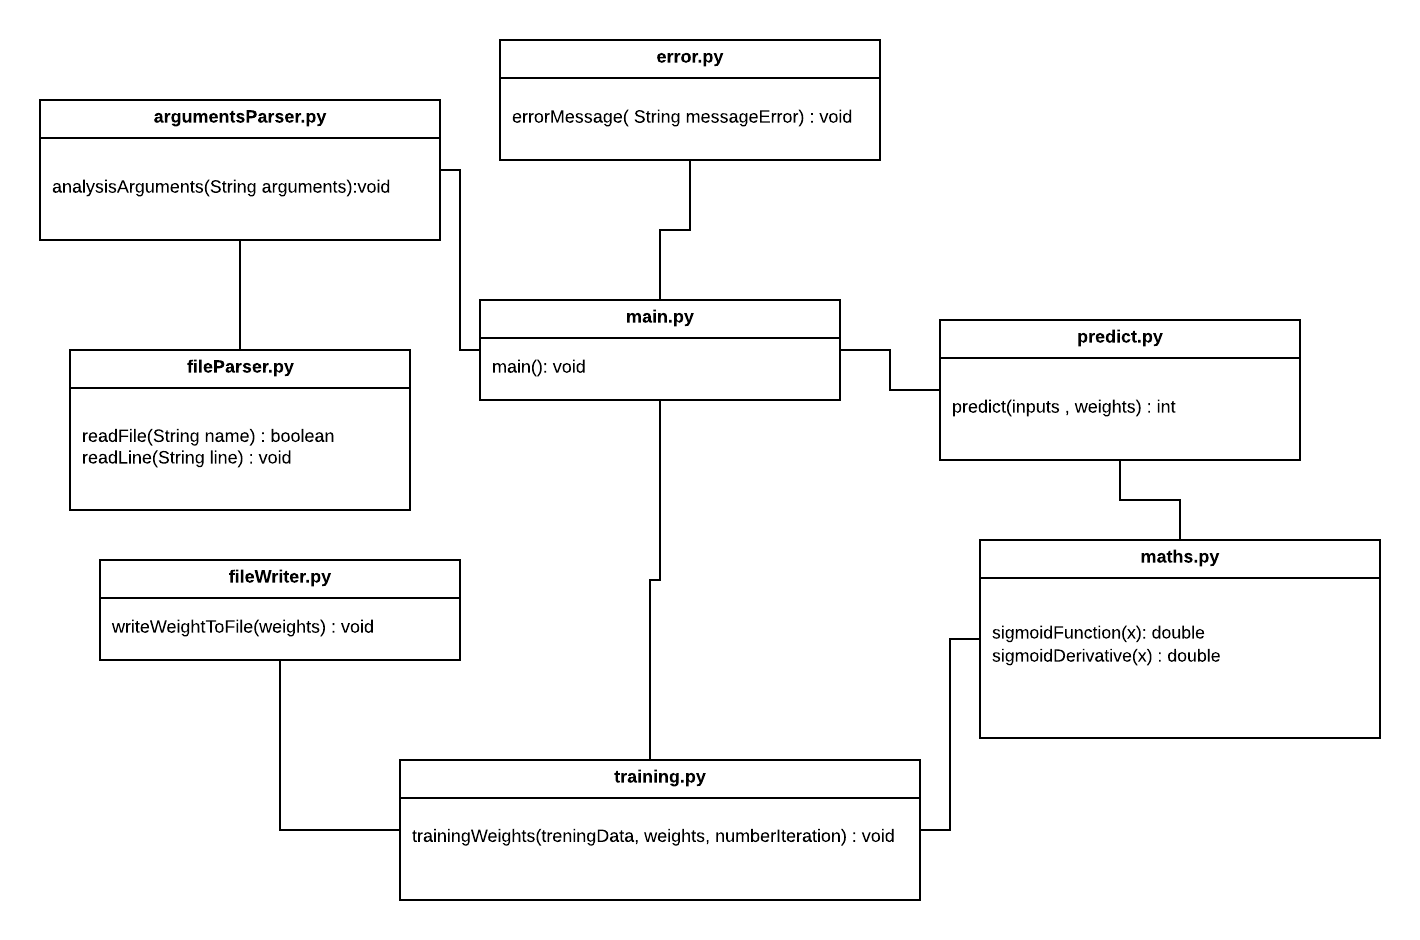
\includegraphics[scale=0.8]{diagram.png}}
\caption{Podstawowy diagram modułow}
\label{fig:image}
\end{figure}

\section{Opis modułów}
\subsection{Moduł argumentsParser}
\hspace*{1 cm} Moduł jest odpowiedzialny za przetwarzanie argumentów z którymi program został uruchamiony. Główną funkcją tego modułu jest funkcja o nazwie \textbf{analysisArguments}.\newline
\hspace*{1 cm} Zadaniem funkcji \textbf{analysisArguments} jest przetwarzanie  argumentów z którymi program był uruchamiony. Funkcja muszi rozpoznać w którym trybie program muszi działać. W zależności od wybranego trybu działania programu funkcja muszi rozpoznawać dodatkowe parametry podane przez użytkownika. Argumenty które muszi rozpoznawać funkcja są następujące:
\begin{itemize}
\item \textbf{-t} argument mówiący o tym że program ma działać w trybie uczenia sieci neuronowej;
\item \textbf{-p} argument mówiący o tym że program ma działać w trybie rozpoznawania języka tekstu;
\item \textbf{-f} argument mówiący że następny argument jest plikiem wejściowym;
\item \textbf{-i} argument mówiący o tym że następnie będzie podana ilość iteracji w ciągu których sieć będzie się uczyć;
\end{itemize}

\subsection{Moduł fileParser}
\hspace*{1 cm}Moduł jest odpowiedzialny za poprawne wczytanie pliku wejściowego podanego przez użytkownika. Główną metodą tego modułu jest funkcja o nazwie \textbf{readLine}. \newline
\hspace*{1 cm}Zadaniem funkcji jest przeczytanie linii tekstu. Podczas czytania linii znak po znaku funkcja ma zliczać wystąpinia poszczegółnych liter w tekscie i zapisywać ilość wystąpień do macierzy. Następnie ta macierz będzie przetwarzana przez sieć neuronową dla rozpaznania języka.

\subsection{Moduł fileWriter} 
\hspace*{1 cm}Moduł jest odpowiedzialny za odpowiednie zapisanie wag które charakteryzują połączenia między neuronami. \newline \hspace*{1 cm} Dla implementacji struktury sieci będzie urzyta lista list w taki sposób, iż główna lista reprezentuje warstwy sieci, a wewnętrzne listy reprezentują neurony w tych warstwach.\newline
\hspace*{1 cm} Przykład zapisania wag w pamięci dla sieci następującej postaci:
\begin{figure}[h]
\centering{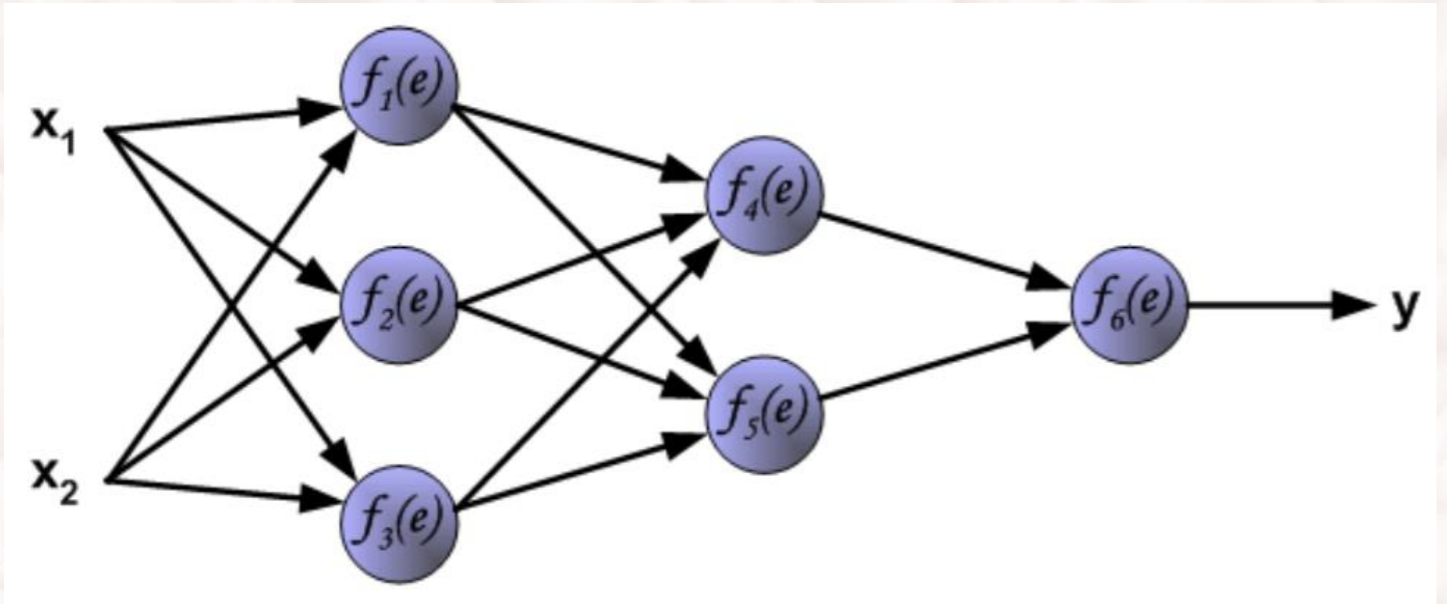
\includegraphics[scale=0.6]{prykladsieci.png}}
\caption{Przykład sieci}
\label{fig:image}
\end{figure}
\begin{verbatim}
Główna lista będzie zawierać poniższe listy
   x1    x2          y1   y2   y3          y4   y5
F1 w11   w12     F4  w41  w42  w43    F6  w64  w65
F2 w21	  w22     F5  w51  w52  w53
F3 w31   w32
\end{verbatim}
\hspace*{1 cm} Funkcja  z modułu \textbf{fileWrite} o nazwie \textbf{writeWieghtToFile} ma odpowiednio zapisać wagi do pliku aby przy użyciu programu dla rozpoznania języka tekstu program mógł z powrotem wczytał wagi.
\subsection{Moduł training}
\hspace*{1 cm} Jeden z najważnejszych modułów programu odpowiadający za uczenie sieci neuronowej czyli za zmianę wag połączeń pomiędzy neuronami. Główną funkcją modulu jest funkcja o nazwie \textbf{trainingWeights}. W funkcja \textbf{trainingWeights} będzie zaimplementowany algorytm  wstecznej propagacji błędów \textit{(ang. backpropagation)}. Dla obliczenia wartości sigmoidalnej funkcji oraz jej pochodnej będą użyte funkcji z modułu \textbf{maths}.
\subsection{Moduł maths}
\hspace*{1 cm} Moduł odpowiadający za matematyczne obliczenia. Główną rolą tego modułu jest wyodrębnienie matematycznych działań od logiki algorytmu. Moduł będzie odpowiadał za obliczenia wartościej sigmoidalnej funkcji oraz jej pochodej. Również w tym modułu będą zaimplementowane funkcje działające na macierzach.  
\subsection{Moduł predict}
\hspace{1 cm}Moduł będzie odpowiadał za rozpoznanie języka. Najważnejszą funkcją tego modułu jest funkcja o nazwie \textbf{preditc}. Funkcja używając wagi oraz dane wejściowe z pliku podanego przez użytkownika będzie przeprowadzać obliczenia poszczególnych wartoścej funkcji aktywacji dla neuronów wszystkich warstw. W wyniku obliczeń uda się stwierdzić czy jest to język na przykład angielski. Poniżej jest pokazany mechanizm obiczenia wartości funkcji aktywacji dla neuronów:
\begin{figure}[h!]
\centering{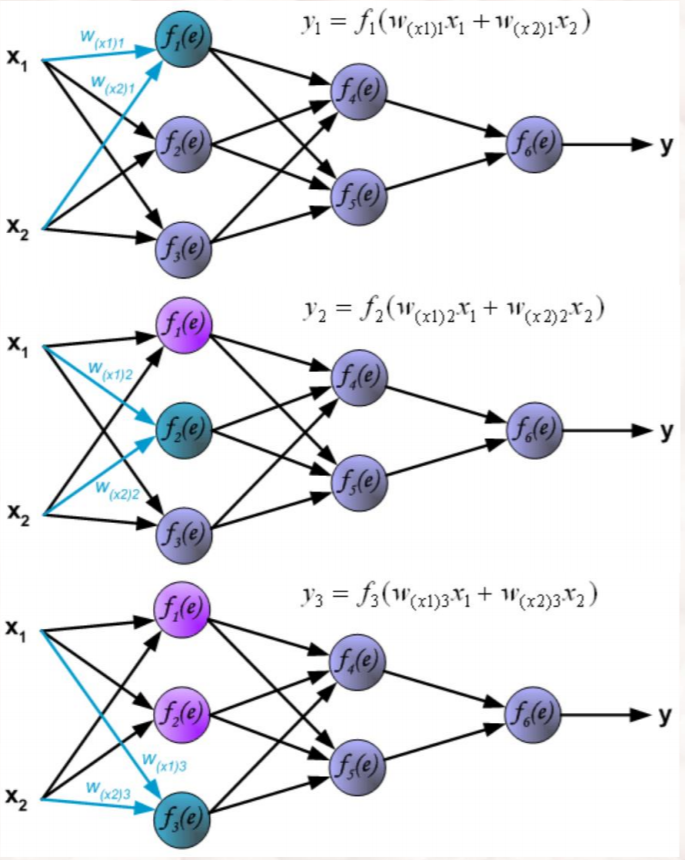
\includegraphics[scale=0.9]{obliczenia.png}}
\caption{Przykład obliczenia funkcji aktywacji}
\label{fig:image}
\end{figure}\newpage
\section{Testy jednostkowe}
\subsection{Moduł fileParser}
\hspace*{1 cm} Test będzie polegać na wczytyniu przez program wcześniej przygotowanego pliku w którym już wiadoma ilość wystąpień poszczególnych liter. Przykładowa zawartość pliku: \newpage
\begin{verbatim}
aaaaaabbbb cc dd mm
\end{verbatim}
\hspace*{1 cm} Test zostanie zaakceptowany gdy program poprawnie przetworzy podany plik wejściowy. Dla przykładowej zawartości pliku muszi powstać odpowiednia lista reprezentująca wystąpienia poszczególnych liter w tekscie. Lista będzie zawierać następujące wartości: 
\begin{verbatim}
6
4
2
0
0
.
.
.
.
2
\end{verbatim}
\subsection{Moduł training}
\hspace*{1 cm} Testowanie tego modułu będzie polegać na tym że zostanie prygotowany zestaw danych w taki sposób że można będzie przewidzieć jakie wartości wag połączeń pomiędzy neuronami ustawią się po jednej iteracji. \newline
\hspace*{1 cm}Test zostanie zaakceptowany jeżeli po jednej iteracji dla przygotowanych danych wagi połąceń będą poprawne. W innym przypadku test zostanie odrzucony. 
\subsection{Moduł predict}
\hspace*{1 cm} Dla testowania tego modułu będzie wygenerowany plik zawierający wagi połączeń pomiędzy neuronami. Test będzie polegał na sprawdzaniu czy moduł  poprawnie rozróżnia język.\newline
\hspace*{1 cm} Test zostanie zaakceptowany gdy na wejście będzie podany tekst w języku angielskim oraz funkcja rozpoznająca język zwróci 1 oraz gdy zostanie podany tekst w języku niemieckim funkcja zwróci 0.
\subsection{Moduł argumentsParser}
\hspace*{1 cm} Moduł zostanie przetestowany podczas implementacji całego programu.
\end{document}